\documentclass[11pt,a4paper]{article}

\usepackage[margin=25mm]{geometry}
\usepackage{amsmath,amssymb,bm}
\usepackage{booktabs}
\usepackage{enumitem}
\usepackage[hidelinks]{hyperref}
\usepackage{tikz}
\usepackage{pgfplots}

\pgfplotsset{compat=1.18}
\usetikzlibrary{arrows.meta,positioning,calc,decorations.markings}

\setlength{\parskip}{0.4em}
\setlength{\parindent}{0pt}

% Tighten section spacing
\usepackage{titlesec}
\titlespacing*{\section}{0pt}{1.2ex plus 0.5ex minus 0.2ex}{0.6ex plus 0.2ex}
\titlespacing*{\subsection}{0pt}{0.9ex plus 0.3ex minus 0.2ex}{0.4ex plus 0.2ex}

% Tighten equation spacing
\AtBeginDocument{%
  \abovedisplayskip=8pt plus 2pt minus 2pt
  \belowdisplayskip=8pt plus 2pt minus 2pt
  \abovedisplayshortskip=4pt plus 1pt
  \belowdisplayshortskip=4pt plus 1pt
}

% Shorthand
\newcommand{\kv}{\mathbf{k}}
\newcommand{\xv}{\mathbf{x}}
\newcommand{\muv}{\bm{\mu}}
\newcommand{\Sigv}{\bm{\Sigma}}
\newcommand{\Fref}{F_\mathrm{ref}}
\newcommand{\Fclean}{F_\mathrm{ref}^\mathrm{clean}}
\newcommand{\Pnoise}{P_\mathrm{noise}}

\title{K-Space Transfer Function Fitting\\for Ensemble Particle Image Velocimetry}
\author{Morgan Taylor}
\date{}

\begin{document}
\maketitle

% ============================================================================
\section{Introduction}
\label{sec:intro}
% ============================================================================

Ensemble particle image velocimetry (PIV) extracts mean displacements and Reynolds stresses from time-averaged correlation planes accumulated over many image pairs.
In physical space, the ensemble cross-correlation is a convolution of the particle image auto-correlation with the velocity probability density function (PDF), requiring a 16-parameter stacked Gaussian fit to separate the two contributions.
This document presents an alternative formulation in wavenumber (k-space), where the particle image shape cancels algebraically, reducing the problem to five parameters: two mean displacement components and three independent elements of the displacement covariance tensor.

The approach proceeds in two stages.
Stage~1 fits the reference spectrum --- the geometric mean of the two auto-correlation power spectra --- to estimate and remove the noise floor.
On warped passes, the interpolation kernel used to shift images colours the noise spectrum; the noise power spectral density (PSD) is computed analytically from the kernel's discrete-time Fourier transform (DTFT) and incorporated into the Stage~1 model.
Stage~2 forms the transfer function by dividing the cross-correlation spectrum by the noise-corrected reference, then fits a Gaussian velocity-PDF model to extract displacements and stresses.

% ============================================================================
\section{Ensemble Correlations and the Reference Spectrum}
\label{sec:correlations}
% ============================================================================

Consider $N$ image pairs $(A_n, B_n)$ acquired at a single interrogation window location.
Three ensemble-averaged spatial correlations are computed:
%
\begin{align}
    R_{AA}(\Delta\xv) &= \frac{1}{N} \sum_{n=1}^{N} \int A_n(\xv)\, A_n(\xv + \Delta\xv)\, \mathrm{d}\xv, \label{eq:raa} \\
    R_{BB}(\Delta\xv) &= \frac{1}{N} \sum_{n=1}^{N} \int B_n(\xv)\, B_n(\xv + \Delta\xv)\, \mathrm{d}\xv, \label{eq:rbb} \\
    R_{AB}(\Delta\xv) &= \frac{1}{N} \sum_{n=1}^{N} \int A_n(\xv)\, B_n(\xv + \Delta\xv)\, \mathrm{d}\xv, \label{eq:rab}
\end{align}
%
where $\Delta\xv$ is the spatial lag.
$R_{AA}$ and $R_{BB}$ are auto-correlations (same exposure with itself); $R_{AB}$ is the cross-correlation (first exposure with second).

Each image decomposes as signal plus noise: $A_n = S_n^A + \eta_n^A$.
In the auto-correlations, the noise correlates with itself, contributing a spike at zero lag that appears as a flat additive floor $N_0$ across all wavenumbers in Fourier space.
In the cross-correlation, the noise terms $\eta_n^A$ and $\eta_n^B$ are statistically independent (separate camera exposures), so their expected cross-correlation vanishes.
This asymmetry --- noise present in auto-correlations but absent from the cross-correlation --- is the fundamental reason noise correction is necessary.

Taking the 2D discrete Fourier transform of each correlation plane yields spectra $F_{AA}(\kv)$, $F_{BB}(\kv)$, $F_{AB}(\kv)$, where $\kv = (k_x, k_y)$ is the wavenumber in cycles per pixel.
The \emph{reference spectrum} is defined as the geometric mean of the auto-correlation magnitudes:
%
\begin{equation}
    \Fref(\kv) = \sqrt{\lvert F_{AA}(\kv)\rvert \cdot \lvert F_{BB}(\kv)\rvert}.
    \label{eq:fref}
\end{equation}
%
The geometric mean treats both exposures symmetrically, handling out-of-plane particle loss and intensity drift.

Without noise, the auto-correlation spectrum of image $A$ is the power spectrum of the average particle image.
For Gaussian particles with $e^{-1/2}$ half-widths $\sigma_x$ and $\sigma_y$, a single particle centred at $\xv_0$ has the Fourier transform
%
\begin{equation}
    \hat{I}_p(\kv) = I_0 \cdot 2\pi\sigma_x\sigma_y \cdot
    \exp\!\bigl(-2\pi^2(\sigma_x^2 k_x^2 + \sigma_y^2 k_y^2)\bigr)
    \cdot e^{-2\pi i\, \kv\cdot\xv_0}.
    \label{eq:ft_particle}
\end{equation}
%
The power spectrum $\lvert\hat{I}_p\rvert^2$ cancels the position-dependent phase (auto-correlations are shift-invariant).
Ensemble averaging over many particles retains the Gaussian spectral shape.
Since $\Fref = \sqrt{\lvert F_{AA}\rvert \cdot \lvert F_{BB}\rvert}$ takes the square root of the power spectra, the exponent halves:
%
\begin{equation}
    \Fref(\kv) \propto \exp\!\bigl(-2\pi^2(\sigma_x^2 k_x^2 + \sigma_y^2 k_y^2)\bigr) + N_0.
    \label{eq:fref_content}
\end{equation}
%
The separate $\sigma_x$ and $\sigma_y$ parameters accommodate astigmatic particle images, which are common in stereo and oblique-viewing configurations.
The noise floor $N_0$ prevents $\Fref$ from decaying to zero at high wavenumbers.

% ============================================================================
\section{The Transfer Function}
\label{sec:transfer}
% ============================================================================

The transfer function is the ratio of the cross-correlation spectrum to the reference spectrum:
%
\begin{equation}
    T(\kv) = \frac{F_{AB}(\kv)}{\Fref(\kv)}.
    \label{eq:transfer}
\end{equation}
%
The cross-correlation spectrum factorises as $F_{AB}(\kv) = \Fclean(\kv) \cdot T_\mathrm{vel}(\kv)$, where $\Fclean$ is the noise-free reference and $T_\mathrm{vel}$ encodes the velocity PDF.
Division by $\Fclean$ cancels the particle image shape, isolating the velocity information:
%
\begin{equation}
    T(\kv) = \frac{\Fclean(\kv) \cdot T_\mathrm{vel}(\kv)}{\Fclean(\kv)} = T_\mathrm{vel}(\kv).
    \label{eq:cancellation}
\end{equation}

Assuming the ensemble velocity PDF is Gaussian with mean $\muv = (\mu_x, \mu_y)$ and covariance $\Sigv$:
%
\begin{equation}
    T(\kv) = \exp\!\bigl(-2\pi^2\, \kv^\top \Sigv\, \kv\bigr)
    \cdot \exp\!\bigl(-2\pi i\, \kv\cdot\muv\bigr),
    \label{eq:tmodel}
\end{equation}
%
where the covariance matrix
%
\begin{equation}
    \Sigv = \begin{pmatrix} \Sigma_{xx} & \Sigma_{xy} \\ \Sigma_{xy} & \Sigma_{yy} \end{pmatrix}
    \label{eq:sigma}
\end{equation}
%
is the Reynolds stress tensor (in pixel$^2$ units).
The five fitted parameters are: $\mu_x$ and $\mu_y$ (mean displacement, from the linear phase of $T$); $\Sigma_{xx}$ and $\Sigma_{yy}$ (normal stresses $\overline{u'^2}$, $\overline{v'^2}$, from the Gaussian decay rate of $\lvert T\rvert$); and $\Sigma_{xy}$ (shear stress $\overline{u'v'}$, from the elliptical tilt of $\lvert T\rvert$).

The advantage over physical-space fitting is direct: $\Sigv$ emerges from the transfer function's decay without requiring a separate estimate of individual particle image widths, eliminating the subtraction $\Sigma = \sigma_{AB}^2 - \sigma_A^2$ that dominates physical-space uncertainty.

% ============================================================================
\section{The Noise Bias Problem}
\label{sec:noise_bias}
% ============================================================================

If $\Fref$ retains the noise floor $N_0$, the measured transfer function becomes
%
\begin{equation}
    T_\mathrm{meas}(\kv) = \frac{F_{AB}(\kv)}{\Fclean(\kv) + N_0}.
    \label{eq:t_biased}
\end{equation}
%
At low wavenumbers where $\Fclean \gg N_0$, the noise is negligible.
At high wavenumbers where $\Fclean \approx 0$, the denominator saturates at $N_0$ and $\lvert T_\mathrm{meas}\rvert$ is artificially suppressed.
The resulting steeper-than-true decay biases the fitted $\Sigv$ upward --- systematically overestimating the Reynolds stresses.
The bias is signal-dependent: windows with weaker seeding or higher noise suffer more.
Accurate noise correction before forming $T(\kv)$ is therefore essential.

% ============================================================================
\section{Interpolation-Induced Noise Colouring}
\label{sec:noise_colouring}
% ============================================================================

On the first pass (no image warping), camera noise $\eta(\xv)$ is spatially uncorrelated with flat power spectral density $P_\eta(\kv) = N_0$.

On subsequent passes, images are warped by a predictor displacement field using an interpolation kernel.
The interpolated image is a weighted sum of neighbouring pixels:
%
\begin{equation}
    A'(\xv) = \sum_j w_j\, A(\xv + \mathbf{d}_j),
    \label{eq:interp}
\end{equation}
%
where $w_j$ are the kernel weights at stencil offsets $\mathbf{d}_j$, which depend on the fractional pixel displacement $f$.
While the signal is faithfully interpolated, the noise is also filtered:
%
\begin{equation}
    \eta'(\xv) = \sum_j w_j\, \eta(\xv + \mathbf{d}_j).
    \label{eq:noise_interp}
\end{equation}
%
The noise PSD of the interpolated image is
%
\begin{equation}
    P_{\eta'}(\kv) = N_0 \cdot \lvert H(\kv, f) \rvert^2,
    \label{eq:noise_psd_general}
\end{equation}
%
where $H(\kv, f)$ is the discrete-time Fourier transform (DTFT) of the kernel weights.

Both the bicubic and Lanczos-3 kernels are separable (applied independently along rows then columns), so the 2D noise PSD factorises exactly:
%
\begin{equation}
    \Pnoise(k_x, k_y) = \lvert H(k_x, f_x) \rvert^2 \cdot \lvert H(k_y, f_y) \rvert^2.
    \label{eq:pnoise_2d}
\end{equation}

\subsection{Bicubic Kernel DTFT}

The bicubic interpolation kernel (Keys, $a = -0.75$, 4-tap) has stencil offsets $\{-1, 0, +1, +2\}$ relative to $\lfloor\text{position}\rfloor$.
The four weights are cubic polynomials in the fractional displacement $f \in [0, 1)$:
%
\begin{align}
    w_{-1} &= a f^3 - 2a f^2 + a f, \notag \\
    w_{\phantom{-}0} &= (a+2) f^3 - (a+3) f^2 + 1, \notag \\
    w_{+1} &= -(a+2) f^3 + (2a+3) f^2 - a f, \label{eq:bicubic_weights} \\
    w_{+2} &= -a f^3 + a f^2, \notag
\end{align}
%
with $a = -0.75$.
The 1D DTFT is
%
\begin{equation}
    H(k, f) = w_{-1}\, e^{+i2\pi k} + w_0 + w_{+1}\, e^{-i2\pi k} + w_{+2}\, e^{-i4\pi k}.
    \label{eq:bicubic_dtft}
\end{equation}

\subsection{Lanczos-3 Kernel DTFT}

The Lanczos-3 kernel (6-tap windowed sinc) has stencil offsets $\{-2, -1, 0, +1, +2, +3\}$.
The weights are
%
\begin{equation}
    w_n = \frac{\operatorname{sinc}(f - d_n)\,\operatorname{sinc}\!\bigl((f - d_n)/3\bigr)}{\displaystyle\sum_m \operatorname{sinc}(f - d_m)\,\operatorname{sinc}\!\bigl((f - d_m)/3\bigr)},
    \label{eq:lanczos_weights}
\end{equation}
%
where $d_n \in \{-2, -1, 0, 1, 2, 3\}$ and $\operatorname{sinc}(x) = \sin(\pi x)/(\pi x)$.
The DTFT is
%
\begin{equation}
    H(k, f) = \sum_n w_n\, e^{-i2\pi k\, d_n}.
    \label{eq:lanczos_dtft}
\end{equation}

\subsection{Symmetric Warp Halving}

The predictor-corrector warping scheme shifts image $A$ by $-\mathbf{d}/2$ and image $B$ by $+\mathbf{d}/2$, where $\mathbf{d}$ is the predictor displacement.
Both images see the kernel at the half-displacement:
%
\begin{equation}
    f_x = \bigl\lvert d_x/2 - \operatorname{round}(d_x/2) \bigr\rvert, \quad
    f_y = \bigl\lvert d_y/2 - \operatorname{round}(d_y/2) \bigr\rvert,
    \label{eq:frac_distance}
\end{equation}
%
giving fractional displacements in $[0, 0.5]$.
Since both auto-correlations see the same noise PSD, the geometric mean~\eqref{eq:fref} inherits a single multiplicative factor of $\Pnoise$.

\subsection{Integer Displacement Limit and Spatial Variation}

When $f = 0$ (integer displacement or no warping), a single kernel tap carries all the weight: $H(k) = 1$ for all $k$, so $\Pnoise = 1$ everywhere --- white noise is recovered.
The model handles this seamlessly without special treatment.

The fractional displacement $f$ varies continuously with the predictor field across the image.
At integer pixel crossings (where $f = 0$), noise is white; between crossings ($f \neq 0$), noise is progressively coloured.
Without correction, this produces characteristic wavy stress artifacts tied to the spatial pattern of integer pixel crossings of the predictor.

\begin{figure}[t]
\centering
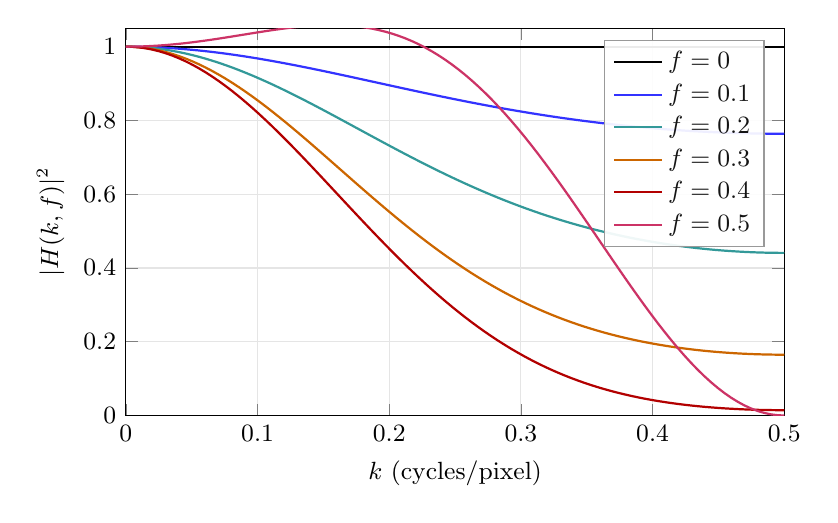
\begin{tikzpicture}
\begin{axis}[
    width=0.82\textwidth,
    height=6.5cm,
    xlabel={$k$ (cycles/pixel)},
    ylabel={$\lvert H(k,f)\rvert^2$},
    xmin=0, xmax=0.5,
    ymin=0, ymax=1.05,
    xtick={0, 0.1, 0.2, 0.3, 0.4, 0.5},
    ytick={0, 0.2, 0.4, 0.6, 0.8, 1.0},
    legend style={at={(0.97,0.97)}, anchor=north east, font=\small,
                  draw=black!40, fill=white, fill opacity=0.92,
                  cells={anchor=west}},
    grid=major,
    grid style={gray!20},
    every axis label/.style={font=\small},
    tick label style={font=\small},
    cycle list name=color list,
]

% f = 0: H = 1
\addplot[thick, black, domain=0:0.5, samples=2] {1.0};
\addlegendentry{$f = 0$}

% For bicubic a=-0.75, compute |H(k,f)|^2 analytically
% H(k,f) = w_{-1} e^{i2pi k} + w_0 + w_1 e^{-i2pi k} + w_2 e^{-i4pi k}
% |H|^2 = (w_{-1}+w_0+w_1+w_2)^2 only at k=0 (=1 always)
% We use the real/imag decomposition:
% Re(H) = w_{-1} cos(2pi k) + w_0 + w_1 cos(2pi k) + w_2 cos(4pi k)
%        = (w_{-1}+w_1) cos(2pi k) + w_0 + w_2 cos(4pi k)
% Im(H) = w_{-1} sin(2pi k) - w_1 sin(2pi k) - w_2 sin(4pi k)
%        = (w_{-1}-w_1) sin(2pi k) - w_2 sin(4pi k)

% f=0.1: a=-0.75, w[-1]=0.063375, w[0]=0.930375, w[1]=-0.000375, w[2]=0.006625
% (w[-1]+w[1]) = 0.063, (w[-1]-w[1]) = 0.06375, w[2] = 0.006625
\addplot[thick, blue!80, domain=0:0.5, samples=100]
    {( 0.063*cos(deg(2*pi*x)) + 0.930375 + 0.006625*cos(deg(4*pi*x)) )^2
    +( 0.06375*sin(deg(2*pi*x)) - 0.006625*sin(deg(4*pi*x)) )^2};
\addlegendentry{$f = 0.1$}

% f=0.2: w[-1]=0.104, w[0]=0.816, w[1]=0.064, w[2]=0.016
\addplot[thick, teal!80, domain=0:0.5, samples=100]
    {( 0.168*cos(deg(2*pi*x)) + 0.816 + 0.016*cos(deg(4*pi*x)) )^2
    +( 0.04*sin(deg(2*pi*x)) - 0.016*sin(deg(4*pi*x)) )^2};
\addlegendentry{$f = 0.2$}

% f=0.3: w[-1]=0.118125, w[0]=0.672375, w[1]=0.178875, w[2]=0.030625
\addplot[thick, orange!80!black, domain=0:0.5, samples=100]
    {( 0.297*cos(deg(2*pi*x)) + 0.672375 + 0.030625*cos(deg(4*pi*x)) )^2
    +( -0.060750*sin(deg(2*pi*x)) - 0.030625*sin(deg(4*pi*x)) )^2};
\addlegendentry{$f = 0.3$}

% f=0.4: w[-1]=0.1, w[0]=0.52, w[1]=0.34, w[2]=0.04
\addplot[thick, red!70!black, domain=0:0.5, samples=100]
    {( 0.44*cos(deg(2*pi*x)) + 0.52 + 0.04*cos(deg(4*pi*x)) )^2
    +( -0.24*sin(deg(2*pi*x)) - 0.04*sin(deg(4*pi*x)) )^2};
\addlegendentry{$f = 0.4$}

% f=0.5: w[-1]=0.0625, w[0]=0.5625, w[1]=0.5625, w[2]=0.0625
% Wait — let me recompute at f=0.5 with a=-0.75:
% w[-1] = -0.75*(0.125) - 2*(-0.75)*(0.25) + (-0.75)*(0.5) = -0.09375 + 0.375 - 0.375 = -0.09375
% Hmm, let me redo: w[-1] = a*f^3 - 2a*f^2 + a*f with a=-0.75, f=0.5
% = -0.75*0.125 + 1.5*0.25 - 0.75*0.5 = -0.09375 + 0.375 - 0.375 = -0.09375
% w[0] = (a+2)*f^3 - (a+3)*f^2 + 1 = 1.25*0.125 - 2.25*0.25 + 1 = 0.15625 - 0.5625 + 1 = 0.59375
% w[1] = -(a+2)*f^3 + (2a+3)*f^2 - a*f = -1.25*0.125 + 1.5*0.25 + 0.75*0.5 = -0.15625+0.375+0.375 = 0.59375
% w[2] = -a*f^3 + a*f^2 = 0.75*0.125 - 0.75*0.25 = 0.09375 - 0.1875 = -0.09375
% Sum = -0.09375 + 0.59375 + 0.59375 - 0.09375 = 1.0 ✓
% (w[-1]+w[1]) = -0.09375+0.59375 = 0.5
% (w[-1]-w[1]) = -0.09375-0.59375 = -0.6875
% w[0] = 0.59375, w[2] = -0.09375
\addplot[thick, purple!80, domain=0:0.5, samples=100]
    {( 0.5*cos(deg(2*pi*x)) + 0.59375 - 0.09375*cos(deg(4*pi*x)) )^2
    +( -0.6875*sin(deg(2*pi*x)) + 0.09375*sin(deg(4*pi*x)) )^2};
\addlegendentry{$f = 0.5$}

\end{axis}
\end{tikzpicture}
\caption{%
Squared frequency response $\lvert H(k,f)\rvert^2$ of the bicubic interpolation kernel (Keys, $a = -0.75$) for fractional displacements $f = 0, 0.1, \ldots, 0.5$.
At $f = 0$ the kernel is a single delta ($H = 1$, white noise).
As $f$ increases toward $0.5$, the kernel distributes weight across multiple taps, progressively suppressing high-frequency noise.
The noise PSD in each spatial direction is $\lvert H(k,f)\rvert^2$; the full 2D PSD is the product of the $x$ and $y$ responses~\eqref{eq:pnoise_2d}.
}
\label{fig:kernel_response}
\end{figure}

% ============================================================================
\section{Joint Reference Spectrum Model (Stage 1)}
\label{sec:stage1}
% ============================================================================

The reference spectrum is modelled as
%
\begin{equation}
    \Fref(\kv) = \Bigl(A \cdot \exp\!\bigl(-2\pi^2(\sigma_x^2 k_x^2 + \sigma_y^2 k_y^2)\bigr) + N_0\Bigr) \cdot \Pnoise(\kv),
    \label{eq:stage1_model}
\end{equation}
%
with four fitted parameters: signal amplitude $A$, particle image widths $\sigma_x$ and $\sigma_y$, and noise amplitude $N_0$.
The noise PSD $\Pnoise$ is computed analytically from the kernel DTFT at the local fractional displacement --- it is known exactly, not fitted.

The key insight is that the interpolation kernel filters everything in the image --- signal and noise together --- so the noise amplitude $N_0$ sits \emph{inside} the bracket with the signal, and $\Pnoise$ multiplies the entire expression.
A naive approach of measuring the noise floor at high wavenumbers would estimate $N_0 \cdot \lvert H(k_\mathrm{high})\rvert^2 \ll N_0$, systematically under-subtracting the noise at low-to-mid wavenumbers where $\lvert H\rvert^2 \approx 1$.
The joint model solves for all four parameters simultaneously from the full spectrum, correctly accounting for the frequency-dependent noise.

\subsection{Fitting Procedure}

\begin{enumerate}[leftmargin=2em]
    \item \textbf{Normalise} $\Fref$ by its DC value $\Fref(\mathbf{0})$ for numerical stability; all parameters are fitted relative to DC.

    \item \textbf{Weighting:} Flat (uniform) weights $w(\kv) = 1$.
    The joint model~\eqref{eq:stage1_model} explicitly separates signal ($A \cdot G$) from noise ($N_0$), so all wavenumbers are informative: low-$k$ points constrain $A$ and $\sigma$, while high-$k$ points where only the $N_0 \cdot \Pnoise$ term remains constrain $N_0$.
    No tapering is necessary.

    \item \textbf{Solver:} Bounded nonlinear least-squares (trust-region reflective) with bounds $A \in [0.01, 10]$, $\sigma_x, \sigma_y \in [0.1, 20]$~px, and $N_0 \in [0, 1]$ (all relative to DC).
\end{enumerate}

The noise-corrected reference spectrum is then
%
\begin{equation}
    \Fclean(\kv) = \max\!\bigl(\Fref(\kv) - N_0 \cdot \Pnoise(\kv),\; \epsilon\bigr),
    \label{eq:fref_clean}
\end{equation}
%
where $\epsilon = \Fref(\mathbf{0}) \times 10^{-8}$ prevents division by zero in Stage~2.

% ============================================================================
\section{Transfer Function Fitting (Stage 2)}
\label{sec:stage2}
% ============================================================================

Stage~1 uses only $\Fref$ (amplitude information, no displacement).
Stage~2 uses the complex transfer function $T(\kv) = F_{AB}(\kv) / \Fclean(\kv)$, which encodes both displacement and stresses.
The two stages share no parameters, preventing degeneracy between noise-floor estimation and velocity-variance estimation.

\subsection{SNR Estimation}

The signal-to-noise ratio is estimated directly from the Stage~1 fit:
%
\begin{equation}
    \mathrm{SNR} = \frac{\lvert\Fclean(\mathbf{0})\rvert^2}{N_0^2}.
    \label{eq:snr}
\end{equation}
%
Since $N_0$ is a parametric estimate of the noise amplitude from the joint model, this ratio measures how far the noise-corrected DC value stands above the noise floor.
The SNR is recorded as a diagnostic but is not used to reject windows --- windows with genuinely insufficient signal will produce small $k_\mathrm{max}$ from the profile threshold and fail at Stage~2 convergence instead.

\subsection{Adaptive Fitting Region}

The fitting region is determined from the noise-corrected reference spectrum $\Fclean$.
The per-axis $k_\mathrm{max}$ is the wavenumber at which $\lvert\Fclean\rvert$ first drops below $1\%$ of its DC value:
%
\begin{equation}
    k_\mathrm{max}^\mathrm{prof} = \max\bigl\{k > 0 \;\big\vert\; \lvert\Fclean(k)\rvert \geq 0.01 \cdot \lvert\Fclean(\mathbf{0})\rvert\bigr\},
    \label{eq:kmax_prof}
\end{equation}
%
sampled along each wavenumber axis (at $k_y = 0$ and $k_x = 0$ respectively).
This is a data-driven bound that adapts to the particle image size and seeding quality of each window independently of the velocity variance.

The profile-based bound is capped at a maximum wavenumber to avoid aliasing and corner artifacts:
%
\begin{equation}
    k_{\mathrm{max},x} = \min\!\bigl(k_{\mathrm{max},x}^\mathrm{prof},\; k_\mathrm{cap}\bigr),
    \label{eq:kmax_combined}
\end{equation}
%
where $k_\mathrm{cap} = 0.35$~cycles/pixel by default.
The fitting region is the ellipse
%
\begin{equation}
    \frac{k_x^2}{k_{\mathrm{max},x}^2} + \frac{k_y^2}{k_{\mathrm{max},y}^2} \leq 1.
    \label{eq:ellipse}
\end{equation}

\subsection{Initial Guesses}

The mean displacement $\muv$ is initialised from the physical-space cross-correlation peak (3-point Gaussian sub-pixel fit), which is immune to phase wrapping for large displacements.
The variances $\hat\Sigma_{xx}$ and $\hat\Sigma_{yy}$ are initialised from 1D log-magnitude regressions along the $k_x$ and $k_y$ axes respectively: since $T(\mathbf{0}) = 1$ after DC normalisation,
%
\begin{equation}
    \ln\lvert T(k_x, 0)\rvert = -2\pi^2 \Sigma_{xx}\, k_x^2,
    \label{eq:1d_regression}
\end{equation}
%
and a linear regression of $\ln\lvert T\rvert$ against $k^2$, forced through the origin, gives $\hat\Sigma_{xx}$.

\subsection{Weighting}

The transfer function fit uses a product of two data-derived weights:
%
\begin{equation}
    w(\kv) = w_\mathrm{snr}(\kv) \cdot w_\mathrm{soft}(\kv).
    \label{eq:stage2_weight}
\end{equation}

The SNR weight is proportional to local signal quality:
%
\begin{equation}
    w_\mathrm{snr}(\kv) = \frac{\lvert\Fclean(\kv)\rvert}{N_0}.
    \label{eq:w_snr}
\end{equation}
%
Where $\Fclean$ is large, the ratio $T = F_{AB}/\Fclean$ is numerically stable; where it is small, dividing amplifies noise, and $w_\mathrm{snr}$ naturally down-weights these regions.

The anisotropic soft decay matches the transfer function's own shape:
%
\begin{equation}
    w_\mathrm{soft}(k_x, k_y) = \exp\!\biggl(-\frac{k_x^2}{k_{0,x}^2} - \frac{k_y^2}{k_{0,y}^2}\biggr),
    \label{eq:w_soft}
\end{equation}
%
where the characteristic wavenumbers are derived from the initial variance estimates:
%
\begin{equation}
    k_{0,x}^2 = \frac{1}{2\pi^2\, \hat\Sigma_{xx}}, \qquad
    k_{0,y}^2 = \frac{1}{2\pi^2\, \hat\Sigma_{yy}}.
    \label{eq:k0}
\end{equation}
%
This weighting decays at the same rate as the model itself: points where $\lvert T(\kv)\rvert$ has decayed significantly contribute less to the fit.
When $\Sigma_{xx} \neq \Sigma_{yy}$, the weighting is anisotropic, matching the elliptical decay of the transfer function.

\begin{figure}[t]
\centering
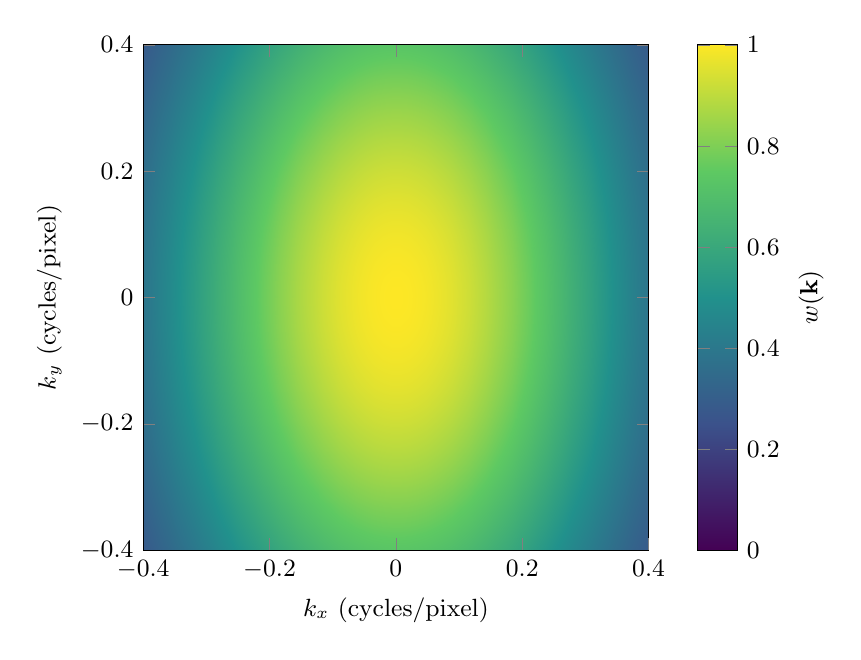
\begin{tikzpicture}
\begin{axis}[
    view={0}{90},
    width=8cm,
    height=8cm,
    xlabel={$k_x$ (cycles/pixel)},
    ylabel={$k_y$ (cycles/pixel)},
    xmin=-0.4, xmax=0.4,
    ymin=-0.4, ymax=0.4,
    xtick={-0.4,-0.2,0,0.2,0.4},
    ytick={-0.4,-0.2,0,0.2,0.4},
    colorbar,
    colorbar style={ylabel={$w(\kv)$}, font=\small},
    colormap={viridis}{
        rgb255(0cm)=(68,1,84);
        rgb255(1cm)=(59,82,139);
        rgb255(2cm)=(33,145,140);
        rgb255(3cm)=(94,201,98);
        rgb255(4cm)=(253,231,37)
    },
    point meta min=0,
    point meta max=1,
    every axis label/.style={font=\small},
    tick label style={font=\small},
]

% Anisotropic Gaussian weight: w = exp(-kx^2/k0x^2 - ky^2/k0y^2)
% Example: Sigma_xx = 0.3 px^2, Sigma_yy = 0.1 px^2
% k0x^2 = 1/(2*pi^2*0.3) = 0.169, k0y^2 = 1/(2*pi^2*0.1) = 0.507
\addplot3[
    surf,
    shader=interp,
    domain=-0.4:0.4,
    domain y=-0.4:0.4,
    samples=60,
]
    {exp(-x^2/0.169 - y^2/0.507)};

\end{axis}
\end{tikzpicture}
\caption{%
Stage~2 soft weighting $w_\mathrm{soft}(\kv)$ in the 2D wavenumber plane for an example with $\Sigma_{xx} = 0.3$~px$^2$ and $\Sigma_{yy} = 0.1$~px$^2$.
The anisotropic Gaussian decay concentrates the fit on wavenumbers where the transfer function signal is strongest.
The shorter extent in $k_x$ reflects the faster decay of $\lvert T\rvert$ along $k_x$ due to the larger streamwise variance.
The full weight~\eqref{eq:stage2_weight} additionally includes $w_\mathrm{snr}$, which further suppresses regions where $\Fclean$ is small.
}
\label{fig:soft_weight}
\end{figure}

\subsection{Five-Parameter Fit}

The transfer function is normalised by its DC value to remove amplitude ambiguity:
%
\begin{equation}
    T_\mathrm{norm}(\kv) = \frac{T(\kv)}{T(\mathbf{0})}.
    \label{eq:tnorm}
\end{equation}
%
The weighted residual for the nonlinear least-squares solver is
%
\begin{equation}
    r(\kv) = w(\kv)\,\bigl[T_\mathrm{norm}(\kv) - T_\mathrm{model}(\kv;\, \muv, \Sigv)\bigr],
    \label{eq:residual}
\end{equation}
%
with $T_\mathrm{model}$ as in equation~\eqref{eq:tmodel}.
The solver minimises $\sum_\kv \lvert r(\kv)\rvert^2$ over the five parameters $(\mu_x, \mu_y, \Sigma_{xx}, \Sigma_{yy}, \Sigma_{xy})$ using trust-region least-squares with geodesic acceleration on the stacked real and imaginary parts.
The normal variances $\Sigma_{xx}$ and $\Sigma_{yy}$ are clamped to zero inside the residual and Jacobian evaluations, ensuring positivity by construction: the optimizer sees a flat cost surface for $\Sigma < 0$, naturally converging to $\Sigma = 0$ when the true variance is near zero (e.g., wall-normal fluctuations near a solid boundary).
The shear stress $\Sigma_{xy}$ is unconstrained (covariance may be negative).

% ============================================================================
\section{Summary}
\label{sec:summary}
% ============================================================================

The complete algorithm for each interrogation window is:

\begin{enumerate}[leftmargin=2em, itemsep=2pt]
    \item Compute $F_{AA}$, $F_{BB}$, $F_{AB}$ by Fourier-transforming the three ensemble correlation planes.

    \item Form the reference spectrum: $\Fref = \sqrt{\lvert F_{AA}\rvert \cdot \lvert F_{BB}\rvert}$.

    \item Compute the noise PSD analytically: $\Pnoise(k_x, k_y) = \lvert H(k_x, f_x)\rvert^2 \cdot \lvert H(k_y, f_y)\rvert^2$ from the interpolation kernel DTFT at the window's half-predictor fractional displacement.

    \item \textbf{Stage~1:} Fit $\Fref = (A \cdot G(\kv;\, \sigma_x, \sigma_y) + N_0) \cdot \Pnoise$ to extract $N_0$.

    \item Subtract the coloured noise: $\Fclean = \max(\Fref - N_0 \cdot \Pnoise,\, \epsilon)$.

    \item Determine the per-axis fitting boundary $k_{\mathrm{max},x}$, $k_{\mathrm{max},y}$ from the profile decay of $\Fclean$~\eqref{eq:kmax_prof}, capped at $k_\mathrm{cap} = 0.35$~\eqref{eq:kmax_combined}.

    \item Form and normalise the transfer function: $T_\mathrm{norm}(\kv) = \bigl(F_{AB}(\kv)\, /\, \Fclean(\kv)\bigr)\, /\, T(\mathbf{0})$.

    \item \textbf{Stage~2:} Fit five parameters $(\mu_x, \mu_y, \Sigma_{xx}, \Sigma_{yy}, \Sigma_{xy})$ from weighted nonlinear least-squares on the complex $T_\mathrm{norm}$ within the elliptical region~\eqref{eq:ellipse}.

    \item Output: mean velocity $\muv$ and Reynolds stress tensor $\Sigv$, extracted directly without particle-shape subtraction.
\end{enumerate}

The method has three key properties.
First, it is seamless across all passes: at pass~0 (no warping), $\Pnoise = 1$ everywhere and the Stage~1 model reduces to a flat noise floor.
No pass-index gating or conditional logic is required.
Second, the noise PSD is computed from the exact analytical DTFT of the interpolation kernel, not estimated from the data.
Third, the Reynolds stresses are extracted directly from the transfer function's Gaussian decay, without requiring a separate estimate of particle image widths or the subtraction of auto-correlation widths from cross-correlation widths.

\begin{figure}[b]
\centering
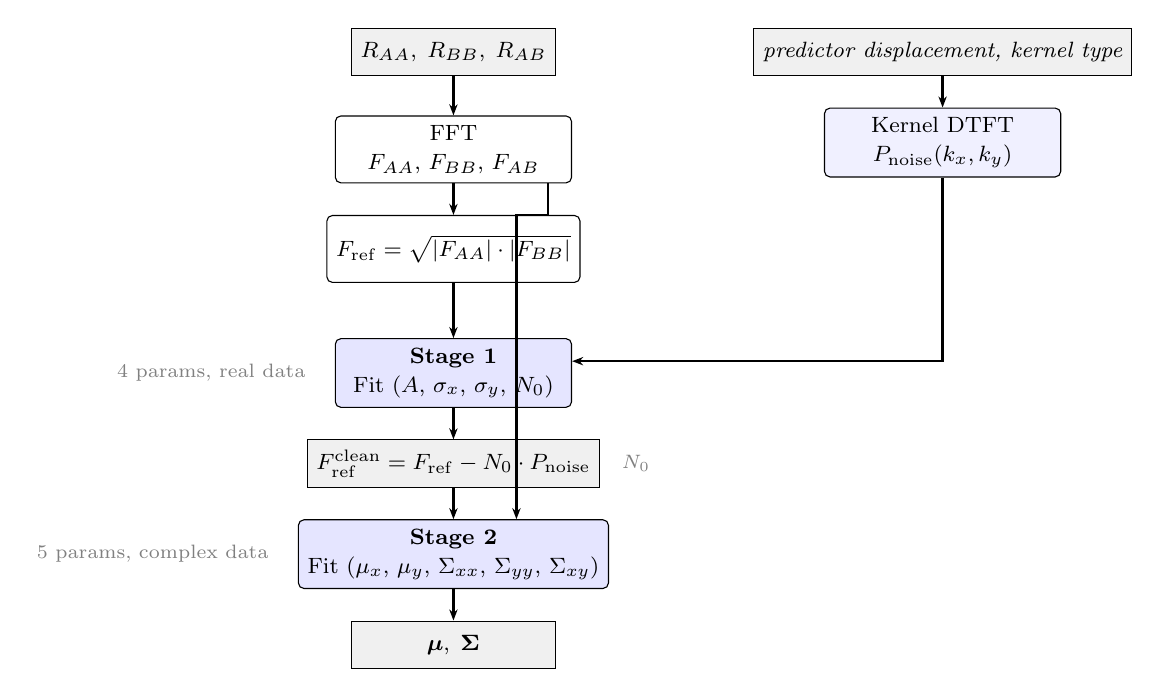
\begin{tikzpicture}[
    node distance=0.4cm and 1.2cm,
    block/.style={rectangle, draw, rounded corners=2pt, minimum height=0.85cm,
                  minimum width=3.0cm, align=center, font=\footnotesize},
    data/.style={rectangle, draw, minimum height=0.6cm,
                 minimum width=2.6cm, align=center, font=\footnotesize\itshape,
                 fill=black!6},
    arrow/.style={-{Stealth[length=4pt]}, thick},
    ann/.style={font=\scriptsize, text=black!50},
]

% Inputs
\node[data] (corr) {$R_{AA},\; R_{BB},\; R_{AB}$};
\node[data, right=2.5cm of corr] (pred) {predictor displacement, kernel type};

% FFT
\node[block, below=0.5cm of corr] (fft) {FFT\\[1pt]$F_{AA},\, F_{BB},\, F_{AB}$};

% Fref
\node[block, below=0.4cm of fft] (fref) {$\Fref = \sqrt{\lvert F_{AA}\rvert \cdot \lvert F_{BB}\rvert}$};

% Pnoise
\node[block, below=0.4cm of pred, fill=blue!6] (pnoise) {Kernel DTFT\\[1pt]$\Pnoise(k_x, k_y)$};

% Stage 1
\node[block, below=0.7cm of fref, fill=blue!10] (s1) {\textbf{Stage 1}\\[1pt]Fit $(A,\, \sigma_x,\, \sigma_y,\, N_0)$};

% Fclean
\node[data, below=0.4cm of s1] (fclean) {$\Fclean = \Fref - N_0 \cdot \Pnoise$};

% Stage 2
\node[block, below=0.4cm of fclean, fill=blue!10] (s2) {\textbf{Stage 2}\\[1pt]Fit $(\mu_x,\, \mu_y,\, \Sigma_{xx},\, \Sigma_{yy},\, \Sigma_{xy})$};

% Outputs
\node[data, below=0.4cm of s2] (output) {$\muv,\;\Sigv$};

% Arrows
\draw[arrow] (corr) -- (fft);
\draw[arrow] (fft) -- (fref);
\draw[arrow] (fref) -- (s1);
\draw[arrow] (pred) -- (pnoise);
\draw[arrow] (pnoise.south) |- ([yshift=0.15cm]s1.east);
\draw[arrow] (s1) -- (fclean);
\draw[arrow] (fclean) -- (s2);
\draw[arrow] ([xshift=1.2cm]fft.south) -- ++(0,-0.4) -| ([xshift=0.8cm]s2.north);
\draw[arrow] (s2) -- (output);

% Annotations
\node[ann, left=0.25cm of s1] {4 params, real data};
\node[ann, left=0.25cm of s2] {5 params, complex data};
\node[ann, right=0.15cm of fclean, anchor=west] {$N_0$};

\end{tikzpicture}
\caption{%
Two-stage pipeline.
Stage~1 estimates the noise floor and particle shape from $\Fref$ alone, using the analytical noise PSD from the interpolation kernel.
Stage~2 divides $F_{AB}$ by the noise-corrected reference $\Fclean$ and fits the transfer function for displacement and Reynolds stresses.
The two stages share no fitted parameters.
}
\label{fig:pipeline}
\end{figure}

\begin{figure}[t]
\centering
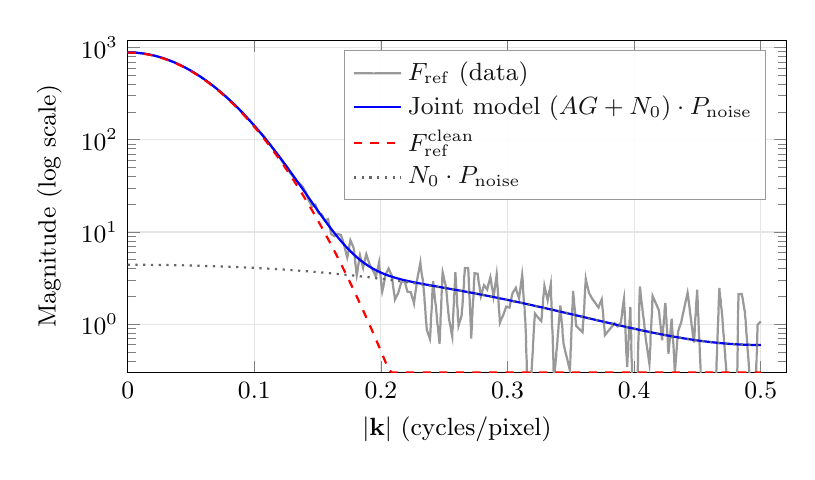
\begin{tikzpicture}
\begin{axis}[
    width=0.82\textwidth,
    height=5.8cm,
    xlabel={$\lvert\kv\rvert$ (cycles/pixel)},
    ylabel={Magnitude (log scale)},
    ymode=log,
    xmin=0, xmax=0.52,
    ymin=0.3, ymax=1200,
    xtick={0, 0.1, 0.2, 0.3, 0.4, 0.5},
    legend style={at={(0.97,0.97)}, anchor=north east, font=\small,
                  draw=black!40, fill=white, fill opacity=0.92,
                  cells={anchor=west}},
    grid=major,
    grid style={gray!20},
    every axis label/.style={font=\small},
    tick label style={font=\small},
]

% Signal parameters: A=1000, sigma=3 px, N0=5
% P_noise for bicubic at f=0.3: approximate as smooth low-pass

% Raw F_ref = (A * Gauss + N0) * P_noise (with jitter)
\addplot[thick, black!40, samples=200, domain=0:0.5,
         decoration={random steps, segment length=1.5pt, amplitude=0.06},
         decorate]
    {( 1000 * exp(-2*3.14159^2 * 9 * x^2) + 5 )
     * ( 0.297*cos(deg(2*3.14159*x)) + 0.672375 - 0.030625*cos(deg(4*3.14159*x)) )^2
     + 2*rand};
\addlegendentry{$\Fref$ (data)}

% Joint model fit: (A*G + N0) * P_noise
\addplot[thick, blue, samples=200, domain=0:0.5]
    {( 1000 * exp(-2*3.14159^2 * 9 * x^2) + 5 )
     * max(( 0.297*cos(deg(2*3.14159*x)) + 0.672375 - 0.030625*cos(deg(4*3.14159*x)) )^2, 0.01)};
\addlegendentry{Joint model $(A G + N_0) \cdot \Pnoise$}

% Noise-corrected: F_ref - N0 * P_noise
\addplot[thick, red, dashed, samples=200, domain=0:0.5]
    {max( ( 1000 * exp(-2*3.14159^2 * 9 * x^2) + 5 )
          * max(( 0.297*cos(deg(2*3.14159*x)) + 0.672375 - 0.030625*cos(deg(4*3.14159*x)) )^2, 0.01)
          - 5 * max(( 0.297*cos(deg(2*3.14159*x)) + 0.672375 - 0.030625*cos(deg(4*3.14159*x)) )^2, 0.01),
          0.3)};
\addlegendentry{$\Fclean$}

% Coloured noise floor: N0 * P_noise
\addplot[thick, black!60, dotted, samples=200, domain=0:0.5]
    {5 * max(( 0.297*cos(deg(2*3.14159*x)) + 0.672375 - 0.030625*cos(deg(4*3.14159*x)) )^2, 0.01)};
\addlegendentry{$N_0 \cdot \Pnoise$}

\end{axis}
\end{tikzpicture}
\caption{%
Radial profile of $\Fref$ for an example window on a warped pass ($f = 0.3$).
The grey curve shows the data; the blue curve is the joint model fit~\eqref{eq:stage1_model}.
The dotted curve shows the coloured noise floor $N_0 \cdot \Pnoise$, which decays at high wavenumbers due to the kernel's low-pass filtering --- a flat noise estimate would over-subtract at high $k$ and under-subtract at mid $k$.
The red dashed curve is the noise-corrected $\Fclean$, which monotonically decays and serves as the denominator for the transfer function in Stage~2.
}
\label{fig:fref_profile}
\end{figure}

\end{document}
